% !TEX encoding = UTF-8 Unicode
\documentclass[a4paper]{article}

\usepackage{listings}
\usepackage{graphicx}
\usepackage[english,serbianc]{babel}
\usepackage[unicode]{hyperref}
\hypersetup{colorlinks,
                 citecolor=Gray,
                 filecolor=Gray,
                 linkcolor=RoyalBlue,
                 urlcolor=RoyalBlue}
\usepackage[usenames,dvipsnames]{color}

% Овако фонт неће бити блед тј. инсталираће
% се квалитетни фонтови за случај да већ нису
\usepackage{type1ec}

% Овако је могуће претраживати и копирати ћирилицу
% из генерисаног документа, независно од хифенације
\usepackage{cmap}
\defaulthyphenchar=127

% Овако је могуће у табели имати текст у два реда
\newcommand{\dvareda}[2][c]{\begin{tabular}[#1]{@{}c@{}}#2\end{tabular}}

% Овако је могуће табеларно представити ауторе
\newcommand{\autor}[2]{\author{\dvareda{#1\\\normalsize{#2}}\medskip}}

% Овако је могуће имати кључне речи
\providecommand{\keywords}[1]
{
	\small	
	\textbf{\textit{Кључне речи ---}} #1
}

% Овако је могуће излитати код
\lstset{ 
  language=R,
  basicstyle=\footnotesize\ttfamily,
  numbers=left,
  numberstyle=\tiny\color{Blue},
  stepnumber=1,
  numbersep=5pt,
  backgroundcolor=\color{White},
  showspaces=false
  showstringspaces=false,
  showtabs=false,
  frame=single,
  rulecolor=\color{black},
  tabsize=2,
  captionpos=b,
  breaklines=true,
  breakatwhitespace=false,
  keywordstyle=\color{RoyalBlue},
  commentstyle=\color{YellowGreen},
  stringstyle=\color{ForestGreen}
} 
\renewcommand\lstlistingname{Скрипт}

% Овако је могуће претпостављати
\newtheorem{hipoteza}{Претпоставка}

\begin{document}

\title{Узорковање слова\\ \small{Семинарски рад у оквиру курса\\Увод у теорију узорака\\Математички факултет, Београд}}

\autor{Лазар Васовић}{mi16099@alas.matf.bg.ac.rs}

\date{23. септембар 2020.}

\maketitle

\abstract{Размотрена је употреба неколико планова узорковања над скупом података који представља велика слова енглеске абецеде, уз праћење релевантних методолошких правила. Велика пажња посвећена је аспектима теме уско повезаним са информатиком, као што су анализа скупа и утицај узорковања на његову класификацију. Посебан значај дат је $R$-у као моћном вишепарадигматском језику. Предложен је статистички заснован метод за одређивање важности предиктора. Све оцене средње вредности обележја од значаја детаљно су упоређене, не само по прецизности, већ и према особинама плана из кога су настале.}

\keywords{слова, узорковање, класификација}

\tableofcontents

\newpage

\section{Увод}

Свако научно истраживање, назависно од теме и обима, представља систематско, планско и објективно испитивање неког проблема, према одређеним методолошким правилима, чија је сврха да се пружи поуздан и прецизан одговор на унапред постављено питање. Обично се састоји од серије логички повезаних фаза, које се простиру од уводног одређивања проблема до закључног представљања резултата.\cite{prez1}

У овом раду спроведено је мини-истраживање над скупом података који представља велика слова енглеске абецеде. Примењена су методолошка правила усвојена на факултетским курсевима Увод у теорију узорака, Статистика и Методологија стручног и научног рада на информатичком смеру Математичког факултета Универзитета у Београду. Једино је скраћена серија фаза, што је последица чињенице да није било прикупљања података, већ је коришћен већ доступан и припремљен скуп ентитета, дакле, у потпуности спремна популација.

Велика пажња посвећена је аспектима теме уско повезаним са информатиком као науком о подацима и њиховој обради, као што су експлоративна анализа скупа и утицај узорковања на његову класификацију. Ово је важно за примене у областима попут истраживања података и машинског учења. Посебан значај дат је и $R$-у као моћном вишепарадигматском програмском језику, при чему је фокус на његовим функционалним, векторским и симболичким концептима, који га издвајају од конкурената у свету савременог статистичког софтвера.

Први циљ спроведеног истраживања био је теоријски, просто стицање увида у преузете податке -- шта они и на који начин представљају (начин генерисања, број и врста обележја) -- као и сазнање о томе који атрибути су међусобно корелисани, да ли подлежу некој од познатих вероватносних расподела и слично. Паралелно са овим циљем, покушан је проналазак одговора на повезано питање примењене природе -- како репрезентативно узорковати, да на основу потпопулације буде могуће направити добар класификациони модел. Идеја је била открити која обележја највише обећавају по питању погађања описаног слова на основну осталих атрибута и то искористити за план узорковања.

\section{Скуп података}

Скуп података „Letter Recognition“ настао је 1991. године за потребе рада „Letter Recognition Using Holland-Style Adaptive Classifiers” америчких научника информатичара Дејвида Џ. Слејта (енгл. \textit{David J. Slate}) и психолога Питера В. Фреја (енгл. \textit{Peter W. Frey}). Обојица се баве разним проблемима вештачке интелигенције и машинског учења, а у поменутом раду су дискутовали прилагодљиве класификаторе.\cite{paper}

Обрађивани подаци јесу они о великим словима енглеске абецеде. Наиме, у питању су црно-беле правоугаоне растерске слике које је потребно препознати као једно од 26 могућих слова. Толики број класа чини овај задатак тешким, за разлику од уобичајеног случаја, када постоје само две односно тек неколико (мали број) категорија.

При генерисању података, употребљено је двадесет различитих фонтова, намерно одабраних тако да обухвате што више различитих стилова и начина писања. Диверзитет и хетерогеност додатно су повећани рандомизованим изобличавањем полазних слика.

Укупно је 20.000 инстанци. Свака од њих је добијена као резултат позива посебно написаног програма за генерисање слике слова. За одабир параметара попут врсте фонта, типа слова, величине слике и фактора изобличења (искривљења), свеобухватности ради, коришћене су равномерно расподељене случајне променљиве/величине.

Додатни детаљи о коришћеним фонтовима и току генераторског програма могу се видети у поменутом раду. Корисно је засад још напоменути да су излаз програма биле слике просечних димензија $45\times45$ пиксела, који су искључиво имали вредности „укључено“ и „искључено“ („да“ и „не“, црно и бело, тачно и нетачно, суштина је да су у питању бинарни пискели, са само две вредности), те да су, упркос изобличењима, према процени ауторâ, сва слова са слика махом била препознатљива људима. Пример добијених слова дат је на слици \ref{slova}.

\begin{figure}[h!]
\begin{center}
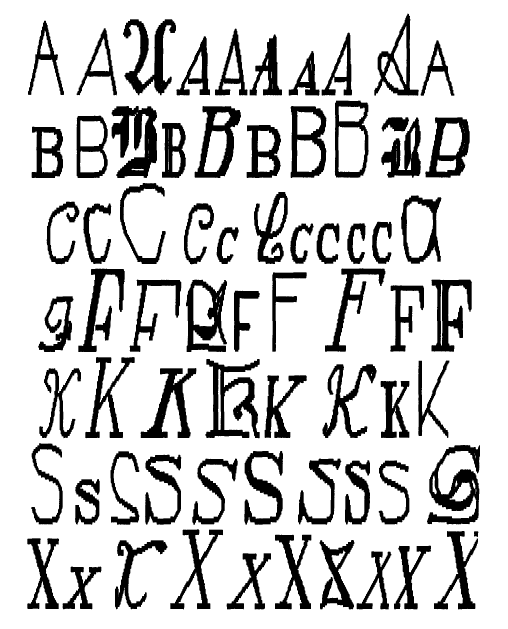
\includegraphics[scale=0.7]{../Slike za rad/Primer slova.png}
\end{center}
\caption{Пример генерисаних слова}
\label{slova}
\end{figure}

Слике, међутим, нису оно што чини овај скуп података, већ низ нумеричких вредности. Ти бројеви су у даљем процесу прављења података добијени систематским читањем слика пиксел по пиксел, те израчунавањем основних статистичких особина расподеле пискела, о чему ће нешто детаљније бити говорено у наставку текста.

\subsection{Опис скупа података}

Скуп података „Letter Recognition“, дакле, чини 20.000 слогова (инстанци, ентитета) распоређених у 26 категорија, које представљају одговарајуће велико слово енглеске абецеде које та инстанца описује. Подаци су јавно и бесплатно доступни на интернет страници репозиторијума за машинско учење Универзитета Калифорније у Ервајну.\cite{data}

Формат података је уобичајени вишедимензиони, у ком различита поља у подацима одговарају различитим мерљивим особинама које су тим пољима (атрибутима, димензијама) представљени. Атрибута има 17, од чега је 16 улазних атрибута квантитативног (нумеричког) типа. Посреди су цели бројеви, мада је дискутабилно да ли их је природније тако посматрати или као категорије, пошто узимају коначан број вредности. Преостаје још један излазни атрибут (класа, тип слова) квалитативног (категоричког), односно именског типа. Јасно је, притом, да је и домен последњег атрибута коначан, те је и он дискретан, попут претходно наведених улазних атрибута. Пример је на слици \ref{skup}.

\begin{figure}[h!]
\begin{center}
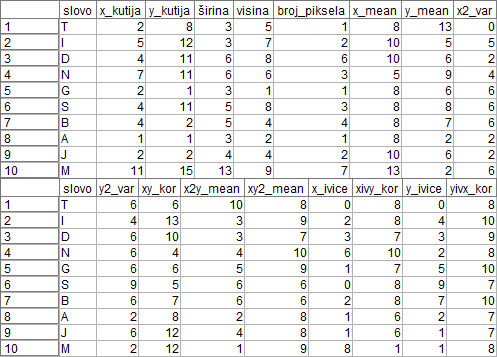
\includegraphics[scale=0.7]{../Slike za rad/Glava skupa.png}
\end{center}
\caption{Глава обрађиваног скупа слова}
\label{skup}
\end{figure}

Оно што овај скуп чини посебно атрактивним јесте чињеница да су сви нумерички атрибути стандардизовани (тј. нормализовани, употреба термина зависи од случаја). Наиме, сваки се налази у целобројном интервалу [0, 15]. Ово је постигнуто линеарним скалирањем, што доприноси компактности података и спречава одређене алгоритме да фаворизују неки атрибут само зато што он има већи распон. Осим тога, на тај начин се олакшава припрема података, односно избегава потреба за претпроцесирањем у контексту скалирања. Ипак, проблем би био покушај опонашања програма за генерисање слова -- не би било јасно како трансформисани добијене сирове податке (слике).

У скупу не постоје недостајуће нити бланко вредности, као ни некоректни нити дуплирани подаци, што додатно олакшава припрему података, као и сам рад са њима. Уз то је свака инстанца независна.

У наставку следи опис сваког атрибута, односно, у случају улазних нумеричких вредности, његовог значења пре сабијања у нормализацијом ограничен интервал. Притом се при помињању координата мисли на уобичајени Декартов координатни систем са почетком у доњем левом углу, у ком $x$ оса расте надесно, док $y$ оса расте нагоре:

\begin{enumerate}
\item slovo -- тип слова, дискретна именска вредност из домена \{A, B, C, D, E, F, G, H, I, J, K, L, M, N, O, P, Q, R, S, T, U, V, W, X, Y, Z\}; представља циљни атрибут, то јест, класу (категорију) инстанце којој је придружена,
\item x\_kutija -- водоравни положај ($x$ координата) центра најмањег правоугаоника који обухвата све „укључене“ пикселе [може се нацртати тако да се сви „укључени“ пиксели налазе у њему],
\item y\_kutija -- усправни положај ($y$ координата) центра те кутије,
\item širina -- ширина (број тј. удео водоравних пиксела) те кутије,
\item visina -- висина (број тј. удео усправних пиксела) те кутије,
\item broj\_piksela -- број тј. удео „укључених“ пиксела на слици,
\item x\_mean -- средња вредност (математичко очекивање) водоравног положаја ($x$ координате) „укључених“ пиксела у односу на центар кутије подељен ширином кутије (негативна вредност за нпр. налево померено „L“),
\item y\_mean -- средња вредност (математичко очекивање) усправног положаја ($y$ координате) „укључених“ пиксела у односу на центар кутије подељен висином кутије (негативна вредност за нпр. надоле померено „L“),
\item x2\_var -- средња вредност квадратне водоравне удаљености (средњеквадратно одступање) „укључених“ пиксела од очекивања из седмог атрибута (дисперзија/варијанса, већа код нпр. хоризонтално раширених „W“ и „M“),
\item y2\_var -- средња вредност квадратне усправне удаљености (средњеквадратно одступање) „укључених“ пиксела од очекивања из осмог атрибута (дисперзија/варијанса, већа код нпр. вертикално раширених „E“ и „K“),
\item xy\_kor -- средња вредност производа водоравног и усправног одступања „укључених“ пиксела од очекивања из седмог и осмог атрибута (корелација, позитивна за линије облика $y = x$, негативна за $y = -x$),
\item x2y\_mean -- средња вредност производа квадратног водоравног и усправног одступања „укључених“ пиксела од очекивања из седмог и осмог атрибута (корелација хоризонталне дисперзије и вертикалног положаја),
\item xy2\_mean -- средња вредност производа квадратног усправног и водоравног одступања „укључених“ пиксела од очекивања из седмог и осмог атрибута (корелација вертикалне дисперзије и хоризонталног положаја),
\item x\_ivice -- средња вредност броја ивица („укључен“ пиксел одмах након [десно од] „искљученог“ или лева ивица/граница/крај слике) при читању (скенирању) слике слева надесно (разликовање нпр. „W“ или „M“  и „I“ или „L“),
\item xivy\_kor -- збир усправних положаја ивица из претходног атрибута (корелација броја вертикалних ивица са хоризонталним положајем, веће за нпр. „Y“),
\item y\_ivice -- средња вредност броја ивица („укључен“ пиксел одмах након [изнад] „искљученог“ или ивица/граница/крај слике) при читању (скенирању) слике од доле нагоре (разликовање нпр. „E“ или „B“  и „I“ или „L“),
\item yivx\_kor -- збир водоравних положаја ивица из претходног атрибута (корелација броја хориз. ивица са верт. положајем).
\end{enumerate}

\subsection{Додатне визуелизације}

За почетак, неопходно је стећи неки утисак о конкретним подацима, као и могућностима за манипулацију њима. Почетни део експлоративне анализе је, једноставности ради, реализован помоћу статистичког пакета \textit{IBM}-овог \textit{SPSS Modeler}-а.\cite{doc} Исто је могло бити урађено помоћу \textit{R}-а, али би захтевало доста кодирања само за увод у причу, тако да се ипак прибегло релативно аутоматизованом приступу. У оквиру овога се само једним кликом могла видети расподела атрибута, број екстрема и аутлајера, као и потврдити већ позната чињеница да су сви подаци исправни и без недостајућих вредности.

У картици за приказ напреднијих визуелизација, дошло се до још занимљивијих резултата. Наиме, најзначајнија је била визуелизација атрибута, што независно (уз опцију аутоматског погађања расподеле), то у паровима (ради разматрања зависности), као и Пирсонова матрица корелација. Помоћу ње је утврђено да су атрибути махом независни у пару, те да највећа корелација (0,62--0,85) постоји између атрибута који представљају димензије, што је и очекивано -- јасно је да ће нпр. ширина и висина кутије бити у тесној вези са $x$ и $y$ координатом њеног центра и слично. Ово је омогућило да се у даљој обради покуша са редукцијом, што ће касније и бити дискутовано.

На слици \ref{raspodela} дат је пример уклапања ширине кутије у нормалну расподелу. На наредним сликама \ref{scatter} и \ref{linzav} дати су дијаграми корелације атрибута са највећом сличношћу, где се уочава њихова средња до јака псеудолинеарна (псеудо због дискретних скокова) зависност.

\begin{figure}[h!]
\begin{center}
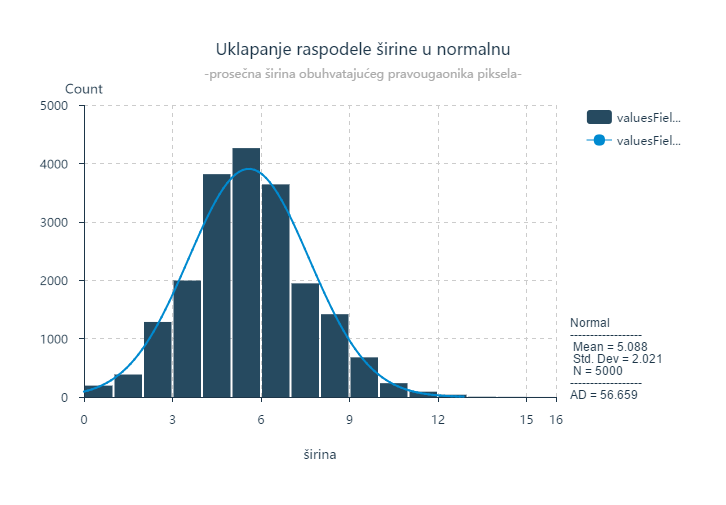
\includegraphics[scale=0.65]{../Slike za rad/Raspodela sirine.png}
\end{center}
\caption{Уклапање расподеле ширине пиксела у нормалну}
\label{raspodela}
\end{figure}

\begin{figure}[h!]
\begin{center}
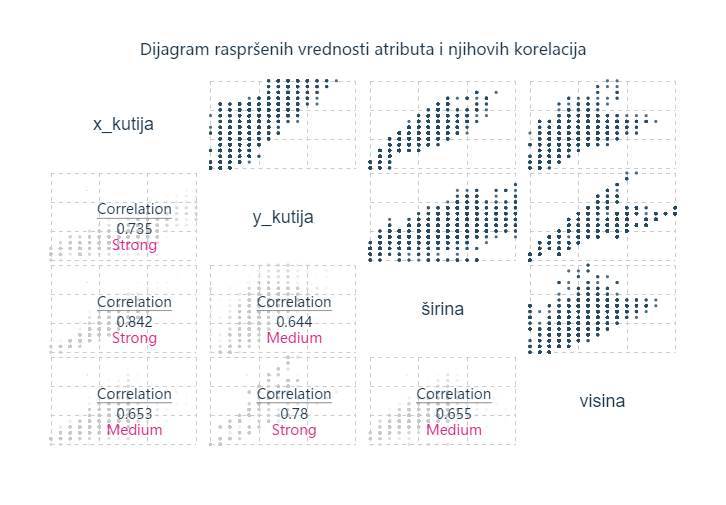
\includegraphics[scale=0.65]{../Slike za rad/Scatterplot.png}
\end{center}
\caption{Приказ парова атрибута са највећом корелацијом}
\label{scatter}
\end{figure}

\begin{figure}[h!]
\begin{center}
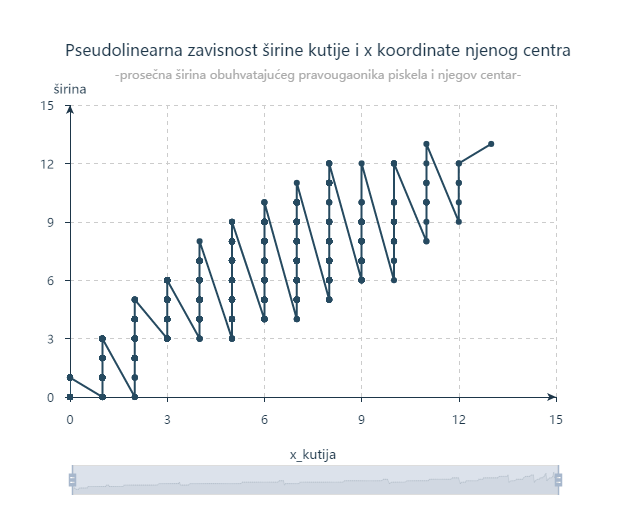
\includegraphics[scale=0.75]{../Slike za rad/Linearna zavisnost.png}
\end{center}
\caption{Приказ пара атрибута са највећом корелацијом}
\label{linzav}
\end{figure}

На слици \ref{barplot} приказан је тракасти дијаграм апсолутних фреквенција циљног атрибута, као начин његове визуелизације и уверавања да су класе релативно равномерно распоређене. Ова слика је добијена помоћу приложеног R скрипта \ref{barlist}, уз наведене функционалне концепте.

\lstinputlisting[caption={barplot.r -- исцртавање тракастог дијаграма},label=barlist]{../R skriptovi/barplot.r}

\begin{figure}[h!]
\begin{center}
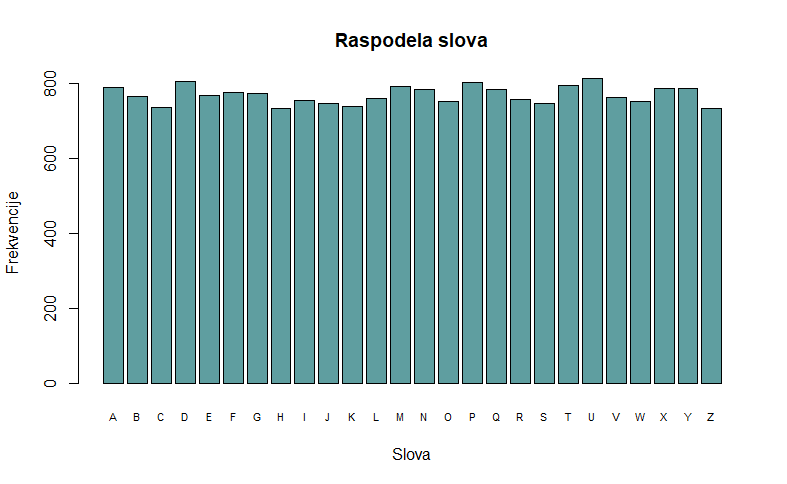
\includegraphics[scale=0.5]{../Slike za rad/Trakasti dijagram.png}
\end{center}
\caption{Тракасти дијаграм категорије}
\label{barplot}
\end{figure}

На крају, одрађена је још једна аутоматска експлорација помоћу \textit{SPSS}-а, овог пута са циљем откривања атрибута који су у високој корелацији са циљним. Како класа није нумеричка, ово није могло бити виђено приликом формирања Пирсонових коефицијената. Резултат овога је важност предиктора, што је списак атрибута уређен по моћи да се на основу њихове вредности одреди категорија ентитета. Приказ је дат на слици \ref{pred}. Како је могуће приметити, као убедљиво најкориснији улазни параметар издваја се четрнаести -- хоризонтална средња вредност броја ивица слова -- тако да је он обележје од значаја.

\begin{figure}[h!]
\begin{center}
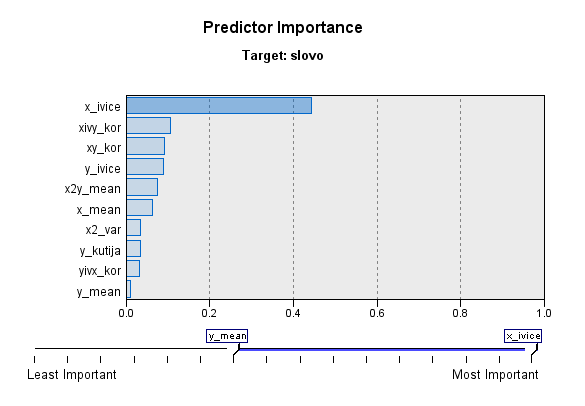
\includegraphics[scale=0.7]{../Slike za rad/Glavni prediktori.png}
\end{center}
\caption{Важност предиктора}
\label{pred}
\end{figure}

Једноставности ради, и ова анализа је, попут претходних у \textit{SPSS}-у, аутоматизована. Представљена је као алгоритам црне кутије, без задирања у конкретну имплементацију, већ само преко резултата. Детаљи би превазишли теорију узорака, па је ипак фокус на простом добијању информацијама који ће бити значајне при даљем раду са базом.

\subsection{Класификација}

Укратко, класификација је проблем препознавања врсте објекта; у конкретном случају -- препознавање које слово представљају неки подаци. Шире гледано, она је пример надгледаног машинског учења, што значи да је заједно са скупом улазних података прослеђен и жељени излаз (класа) за сваку инстанцу. Алгоритми класификације приликом учења модела (укалупљивања података у модел) знају која инстанца представља које слово. На основу виђених података покушава се формирање представе о узрочно-последичним односима у обрађеном скупу података, као и уопштавање закључака на невиђене податке, са циљем да излазни модел са великом прецизношћу разликује слова према њиховим особинама. Крајњи резултат тестира се на контролним подацима -- оним који нису учествовали у тренирању.

Како је најављено да ће планови узорковања бити коришћени за класификацију скупа, ваља проценити предиктивну моћ модела направљеног над целом популацијом. То је и урађено скриптом \ref{klasif}. Притом је као алгоритам за прављење модела коришћен метод потпорних вектора (енгл. \textit{support-vector machine}, SVM). Овај метод заснован је на статистичкој теорији учења и на идеји векторских простора. Модел је формула на основу које се израчунава класа. Алгоритам налази раздвајајућу хиперраван која раздваја категорије унутар векторског простора података, при чему максимизује размак између хиперравни и најближих јој инстанци које раздваја. Један је од најкомплекснијих метода надгледаног машинског учења, али је зато врло успешан. На обрађеном скупу података постигнута је прецизност од 96,24 \%.

\lstinputlisting[caption={klasif.r -- модел над целом популацијом},label=klasif]{../R skriptovi/klasif.r}

Наравно, ово је најпростији случај, без поделе на тренинг и тест скуп, тако да је у питању својеврсна горња граница прецизности. У наставку ће се подела вршити изабраним плановима узорковања, а циљ ће бити задржати што већу прецизност упркос мањем улазу.

\section{Узорковање}

Узорковање је извлачење подскупа популације. Тај подскуп, очекивано, садржи извесне ентитете који потичу из
популације, на бази чијег проучавања се изводе закључци о читавој популацији. Узорковање је важно, чак и када је цела популација (цензус) доступна.\cite{lohr} Постоји већи број предности делимичног испитивања -- мања цена, већа брзина и, можда најзначајније, контрола тачности (нпр. у машинском учењу је узорак тренинг скуп, док је остатак популације тест скуп).

Посматрано кроз статистичку терминологију, сваки скуп конкретних вредности обележја које описују једно слово назива се јединица посматрања (често је то и јединица узорковања), док су сва слова заједно управо популација. Величина популације је 20.000, док је оквир за одабир узорка произвољног обима база дата у формату запетом раздвојених вредности (једна \textit{CSV} датотека). Ознака јединице је индекс ентитета у скупу, пошто он заправо и није неуређени скуп, већ уређени низ. О природи 17 обележја већ је детаљно дискутовано.

\subsection{Прост случајан узорак}

Прост случајан узорак је једноставан план узорковања у коме је јединица посматрања једнака јединици узорковања.\cite{prez2} Из популације се сукцесивно узима ентитет по ентитет, све док се не достигне жељени обим узорка. Све инстанце имају једнаку вероватноћу да буду изабране у неком кораку, при чему понављања могу или не морају бити дозвољена. Најчешће се узоркује преко ознака, у конкретном случају -- индекси слова. Уобичајене ознаке су $N$ за величину популације, а $n$ за обим узорка. Случајан избор реализује се помоћу генератора случајности, што је овде $R$-ов програмски генератор псеудослучајних бројева. Приликом закључивања се користи приступ заснован на методу одабира узорка -- популација је фиксирана (детерминистичка, све се тачно налази у датотеци), само вредности њених обележја нису позната. Једина случајност, дакле, лежи у одабиру узорка.

Како је при уводним разматрањима утврђено да хоризонтална средња вредност броја ивица слова (четрнаести атрибут) има највећу предиктивну вредност, може се претпоставити да ће солидан успех донети узорак који има сличне статистичке особине тог обележја.

\begin{hipoteza}
Класификациони модел направљен над узорком који чува расподелу четрнаестог атрибута постиже већу прецизност од оног направљеног над узорком који ту расподелу не чува.
\end{hipoteza}

Први покушај је, стога, осигурати се да узорак испуњава изнесену претпоставку. Конкретно се може посматрати средња вредност обележја. Њена непристрасна тачкаста оцена је узорачка средња вредност $\overline{Y}$. Ова оцена није прецизна за узорке малог обима, при чему је тачкаста оцена њене дисперзије $\frac{\overline{S}^2}{n}(1 - \frac{n}{N})$ за прост случајан узорак без понављања, а без фактора корекције $\frac{\overline{S}^2}{n}$ за узорак са понављањем. Двострани приближни интервал поверења популацијске средње вредности је $\overline{Y} \pm z_{1 - \frac{\alpha}{2}}\sqrt{\hat{\sigma}^2}$, при чему је $\hat{\sigma}^2$ оцена дисперзије.

Идеја је да апсолутна разлика између оцене и праве популацијске вредности буде што мања. Може се показати да је $n_0 = (\frac{\sigma z_{1-\frac{\alpha}{2}}}{\Delta})^2$ добра доња граница обима узорка са понављањем када се ради са популацијском средњом вредношћу, док се $\frac{1}{\frac{1}{n_0} + \frac{1}{N}}$ користи код узорка без понављања. Притом је $\sigma$ популацијска ст. грешка, $\alpha$ дозвољена грешка прве врсте (поверење $1 - \alpha$), $\Delta$ дозвољена апсолутна грешка, а $z$ одговарајући квантил стандардне нормалне распоределе.

Узорковање без понављања је одрађено у скрипту \ref{srswor}. Изабрана је прилично конзервативна дозвољена апсолутна грешка, уз висок ниво поверења 95 \%. Како би се одредио адекватан обим узорка, спроведено је пилот истраживање над сточланим узорком, што је омогућило процену дисперзије. Испоставља се да је оцена средње вредности обележја од значаја одлична -- узорачке вредности врло су блиске популацијским, са апсолутном грешком мањом од највеће дозвољене, а дисперзија оцене је мала. И добијени интервал поверења је, упркос високом  задатом степену поверења, прилично узак, при чему је, очекивано, успешно обухватио популацијску средњу вредност. На крају, над овим узорком од 3199 инстанци (свака шеста или седма) направљен је класификациони модел који погађа добрих 87,68 \% слова.

\lstinputlisting[caption={srswor.r -- модел над \textit{SRSWOR} узорком},label=srswor]{../R skriptovi/srswor.r}

Узорковање са понављањем је одрађено у скрипту \ref{srswr}. Код је сличан као за верзију без понављања. Ипак, овде свако извлачење даје реализацију случајне величине независне од осталих, тако да нема фактора корекције (отклона) у формулама, нити теоријске потребе за проширењем централне граничне теореме зарад решавања проблема коначне популације (суперпопулација и слично). Шире гледано, бутстреп (енгл. \textit{bootstrap}) методе -- статистички поступци засновани на узорцима са понављањем -- популарне су у машинском учењу. Не само што су у позадини лакше за имплементацију (нема провере јединствености), већ се испоставља да често дају боље резултате од метода без понављања. Над узорком од 3808 инстанци (свака пета или шеста) направљен је класификациони модел који погађа 88,29 \% слова. Редуковани узорак од 3445 инстанци (уклањање дупликата) учествовао је у прављењу врло сличног модела са прецизношћу 88,11 \%.

\lstinputlisting[caption={srswr.r -- модел над \textit{SRSWR} узорком},label=srswr]{../R skriptovi/srswr.r}

Засад се чини да предложени план узорковања даје добре резултате по питању прецизности добијеног класификационог модела. Проценат погођених слова свеукупно веома је висок код модела направљених над узорцима који чувају расподелу обележја од значаја. На тренинг скупу је, очекивано, још већи, док је на тест скупу сличан просечној вредности. Прецизност опада повећањем дозвољене апсолутне грешке оцене, али је тада и обим узорка мањи. За проверу изнесене претпоставке, неопходно је још показати како се понашају други модели -- они који не чувају расподелу хоризонталног броја ивица.

\subsection{Узорак са неједнаким вероватноћама}

Узорак са неједнаким вероватноћама је још један једноставан план узорковања, с тим што код њега јединица посматрања није нужно једнака јединици узорковања.\cite{prez4} И у овом случају важе опште тврдње изнесене за прост случајан узорак, са главном разликом да овде свака инстанца има засебну вероватноћу извлачења у неком кораку.

Ред је вратити се на претходну претпоставку. Сада је циљ формирати узорак који не чува расподелу обележја од значаја и упоредити га са оним који чува. За те потребе може се формирати узорак са неједнаким вероватноћама, при чему вероватноћа одабира намерно расте удаљавањем од популацијске средње вредности. На овај начин очекује се веће одступање узорачке средње вредности од популацијске, као и већа узорачка варијанса. Резултат се може оценити неком од познатих непристрасних оцена средње вредности код овог плана узорковања -- Хансен-Хурвицовом $\frac{1}{Nn} \sum_{k \in R} \frac{y_k}{\psi_k}$, Хорвиц-Томпсоновом $\frac{1}{N} \sum_{k \in S} \frac{y_k}{\pi_k}$ или Хајековом $\frac{\sum_{k \in S} \frac{y_k}{\pi_k}}{\sum_{k \in S} \frac{1}{\pi_k}}$, при чему су $\psi$ вероватноће извлачења у неком кораку, $\pi$ вероватноће укључења првог реда, $R$ узорак, а $S$ редуковани узорак без понављања. Познате су и тачкасте оцене дисперзија претходних оцена, и оне су израчунате у коду, иако, једноставности ради (велике су формуле), нису наведене у тексту.

Овакво узорковање са понављањем одрађено је у скрипту \ref{upswr}. Коришћен је обим узорка израчунат при раду са простим случајним узорком. Вештачки уведене неједнаке вероватноће одабира квадратно расту са удаљавањем обележја од значаја од његове средње вредности, како би се добио узорак који не чува расподелу тог атрибута. Знајући расподелу при одабиру, све три оцене показале су се као одличне при погађању популацијске средње вредности. Веома су прецизне и са малом варијансом, упркос великој узорачкој дисперзији обележја. Ипак, алгоритми класификације не користе податак о вероватноћи одабира, већ само на основу улазних инстанци праве модел, сматрајући да су добили репрезентативан узорак. Тако је на основу узорка од 3808 ентитета добијена прецизност од само 68,785 \% (упоредити са претходних 88,29 \% за исти обим узорка), док је над редукованим узорком од 2781 инстанце постигнута слична прецизност 68,045 \% (претходно 88,11 \%, додуше, са мањом редукцијом, због мањег удела дупликата).

\lstinputlisting[caption={upswr.r -- модел над неједнаким вероватноћама},label=upswr]{../R skriptovi/upswr.r}

Верзија без понављања одрађена је у скрипту \ref{upswor}. Ситуација је слична као код верзије са понављањем, уз разлику да није оцењивана популацијска вредност, пошто прва оцена захтева узорак са понављањем, док друге две захтевају познате вероватноће укључења, које није лако израчунати. На основу узорка од 3199 инстанци добијена је прецизност од 68,3 \% (упоредити са претходних 87,68 \% код простог случајног узорка, одабраног тако да чува расподелу обележја од значаја).

\lstinputlisting[caption={upswor.r -- модел над неједнаким вероватноћама},label=upswor]{../R skriptovi/upswor.r}

Када се све узме у обзир, могло би се закључити да је предложена хипотеза тачна, те да класификациони модел направљен над узорком који чува расподелу четрнаестог атрибута заиста постиже већу прецизност од оног направљеног над узорком који ту расподелу не чува. Не само то, већ би се могао предложити општи метод за одређивање обележја од значаја за проблем класификације. Наиме, у случају да није познато који је атрибут у најтешњој вези са циљном класом, имало би смисла проћи кроз сваки, при чему би се спровели следећи кораци:

\begin{enumerate}
\item извлачење простог случајног узорка одговарајућег обима који чува расподелу текућег обележја и прављење модела,
\item извлачење узорка са неједнаким вероватноћама осмишљеним тако да „кваре“ расподелу текућег обележја и прављење модела,
\item поређење прецизности -- разлика указује на предиктивни значај обележја, и то вероватно тако да је већа разлика важнија.
\end{enumerate}

\subsection{Количничко и регресионо оцењивање}

Количничко оцењивање, поред интересног атрибута $Y$, узима у обзир вредности помоћних обележја која су висококорелисана са обележјем од значаја, нпр. неког $X$.\cite{prez5} На тај начин се боље искоришћавају подаци и добијају оцене са често мањом дисперзијом него када се посматра само интересни атрибут. У најједноставнијем облику, израчуна се однос (количник) узорачких средњих вредности $R = \frac{\overline{Y}}{\overline{X}}$ или тотала, а затим се о непознатим параметрима расподеле $Y$ на целој популацији закључује преко познатих параметара $X$, нпр. $\hat{\tau}^R_y = \tau_x R$, где је $\tau_x$ познати популацијски тотал помоћног обележја, док је $\hat{\tau}^R_y$ количничка оцена тотала обележја од значаја. Осим мање дисперзије, предност овог приступа је и могућност оцењивања када није позната величина популације. Мана је што су оцене благо пристрасне, али су ипак асимптотски непристрасне, те су добре за веће узорке.\cite{cochran}

Регресионо оцењивање иде корак даље. И овде се предлаже техника којом се побољшава прецизност оцена непознатих популацијских параметара главног обележја $Y$, коришћењем помоћног обележја $X$ које је у корелацији са $Y$, уз додатак да је ограничење слободније -- прихватљиве су и линеарне везе по правама које не пролазе кроз координатни почетак, док је код количничког оцењивања то неопходно.\cite{prez6} Главни резултат овог приступа је тачкаста оцена средње вредности $\hat{m}^{lr}_y = \overline{Y} + b (m_x - \overline{X})$, са погодном унапред одабраном константом (алтернативно статистиком) $b$ и другим познатим ознакама.

Овакво оцењивање, међутим, није претерано корисно када је у питању проучавани скуп слова. Иако је обележје од значаја нумеричког типа, категорије нису, тако да нема смисла погађати их на овај начин. С друге стране, сама идеја која стоји иза количничког и регресионог приступа -- руковање висококорелисаним паровима атрибута -- врло је важна у машиском учењу, па је и размотрена у наставку.

Често је превише захтевно радити са свим обележјима неког скупа података. Тада се прибегава својеврсном вертикалном узорковању -- бира се подскуп атрибута уместо подскупа ентитета. Овај процес назива се димензиона редукција,\cite{mitic} док је њен аспект обрађен у овом раду такозвани одабир карактеристика (енгл. \textit{feature selection}). Једноставна идеја заснива се на искључивању атрибута који су у високој корелацији са неким другим обележјем. Претпоставка је да би се тај атрибут могао израчунати на основу других (идеја еквивалентна оној из количничког и регресионог оцењивања), те да из тог разлога не доприноси варијетету података, што даље повлачи да није користан у прављењу класификационог модела, те да се може избацити.

\begin{hipoteza}
Класификациони модел направљен над скупом података из кога су искључена висококорелисана обележја (вертикални узорак) постиже исту прецизност као онај направљен над целим скупом, док искључивање некорелисаних обележја смањује прецизност.
\end{hipoteza}

Ово је проверено у скрипту \ref{corr}, над целокупним скупом и сва три плана простог случајног узорка. Искључени су други, четврти, пети и шести атрибут, пошто се показало да су у тесној вези (коефицијент корелације већи од 0,75) са првим и трећим обележјем, тј. да се могу преко њих израчунати, те да не доприносе варијабилности. Модел над целим скупом постигао је прецизност 94,89 \% (упоредити са 96,24 \% пре редукције). Модел над простим случајним узорком без понављања погодио је 85,785 \% слова (упоредити са 87,68 \%). Модел над простим случајним узорком са понављањем био је успешан у 86,725 \% случајева (упоредити са 88,29 \% пре редукције), док је над редукованим узорком прецизност била 86,185 \% (упоредити са полазних 88,11 \%).

\lstinputlisting[caption={corr.r -- модел над редукованим подацима},label=corr]{../R skriptovi/corr.r}

Свеукупно гледано, прецизност је за све реализоване планове узорковања опала за мање од 2 \%, што је углавном занемарљиво мало -- уколико је прихватљиво 87 \% погодака, прихватљиво је у 85 \%. Притом је димензија проблема осетно смањена -- 16 улазних атрибута сведено је на 12 (уштеда од једне четвртине) -- што двоструко убрзава алгоритам класификације. Остаје испитивање другог дела хипотезе.

Искључивање нискокорелисаних атрибута, које није могуће исправно израчунати преко осталих (аналогно примени количничке или регресионе оцене на пар обележја са коефицијентом корелације око 0,3 или мањом), урађено је у скрипту \ref{corrlos}. Очекивано, губитак у прецизности је велики -- око 11 \% -- што није прихватљива цена редукције.

\lstinputlisting[caption={corrlos.r -- модел над редукованим подацима},label=corrlos]{../R skriptovi/corrlos.r}

На основу виђеног, могуће је закључити да је полазна претпоставка тачна -- озбиљно класификациони модел направљен над скупом података из кога су искључена висококорелисана обележја (вертикални узорак) постиже сличан успех као онај направљен над целим скупом, док искључивање некорелисаних обележја смањује прецизност -- уз напомену да то важи уз одређени степен грешке. Даље истраживање могло би бити усмерено на прецизно оцењивање тог одспутања, што због обима није урађено у овом раду. Грешка од 2 \%, примећена на обрађиваном скупу слова, није велика и има смисла да би и на осталим скуповима била подједнако прихватљива и релативно занемарљива.

\subsection{Стратификован (раслојен) узорак}

Стратификацијом (раслојавањем) популације на основу вредности помоћног обележја за које се сматра да је у вези са атрибутом од значаја добија се скуп међусобно дисјунктних потпопулација (слојева, стратума). Након тога се из сваког слоја могу бирати узорци унапред одређеног обима. Притом су одабири из различитих стратума независни и не нужно начињени према истом плану узорковања. Резултат описаног поступка јесте стратификован (раслојен) узорак.\cite{prez7}

Под претпоставком да се подузорак из сваког слоја извлачи вероватносним методом, непристрасна тачкаста оцена популацијског тотала једнака је збиру оцена за сваки стратум, са дисперзијом једнаком збиру појединачних дисперзија (последица независности). Закључивање о средњој вредности и интервалима поверења аналогно је, као код других планова, сагласно са везом $m = \frac{\tau}{N}$ и распоном $\overline{Y} \pm z_{1 - \frac{\alpha}{2}}\sqrt{\hat{\sigma}^2}$.

Овакав план узорковања, у случају стварне корелације посматраног и помоћног обележја, често смањује вероватноћу одабира нерепрезентативних узорака, што је предност у свакој примени. Оцене непознатих параметара тада су прецизније, а омогућено је и закључивање о појединачним слојевима. Некада је чак и једноставније или јефтиније узорковање по слојевима него на целој популацији одједном. Поред корелације обележја, пожељне особине стратума су релативна хомогеност унутар слојева и релативна хетерогеност између слојева. То се обично подразумева када је подела на стратуме природна.

Поставља се питање како дефинисати слојеве и одредити њихов број, а одговор у суштини зависи од проблема тј. скупа података који се проучава. На примеру обрађиваних слова, како је четрнаести атрибут обележје од значаја и како је он одређен као предиктор високе важности, природно је стратификовати према типу слова које ентитет описује. Тиме је прецизно одређено 26 независних потпопулација.

\begin{hipoteza}
Узорак раслојен према типу слова боље оцењује средњу вредност четрнаестог атрибута до простог случајног узорка. Додатно, класификациони модел направљен над тим узорком постиже већу прецизност од оног формираног над простим случајним узорком.
\end{hipoteza}

Други важан проблем јесте одређивање расподеле узорка по појединачним стратумима. Најпростији одговор лежи у пропорционалном распореду -- обим подузорка је сразмеран обиму слоја. Нешто сложенији одговори испуњавају додатан захтев за смањеном дисперзијом, а међу њима је Нејманов оптимални распоред, који предлаже обиме $n_h = n \frac{N_h \sigma_h}{\sum_{l \in H} N_l \sigma_l}$ за сваки слој $h$, где је $H$ скуп свих стратума $l$. Очигледно, идеја је да више ентитета потиче из већих и/или распршенијих потпопулација, чиме је боље очувана варијабилност полазног скупа.

Напослетку, остаје одабир обима узорка $n$ таквог да минимизује дисперзију оцене, нпр. кад се процењује средња вредност. Наивна идеја је да се користи исти обим као код нпр. простог случајног узорка или ког већ плана који се користи за одабир подузорка унутар стратума. Боља замисао узима у обзир специфичне варијансе сваког појединачног стратума. Тако се као обим узорка може одабрати $n = \upsilon (\frac{z_{1-\frac{\alpha}{2}}}{\Delta})^2$, при чему је оцена $\upsilon = \frac{1}{N} \sum_{h \in H} N_h \sigma_h^2$, док су остале ознаке познате.

Стратификовано узорковање са пропорционалним распоредом код кога се подузорци из сваког стратума извлаче простим случајним узорковањем без понављања одрађено је у скрипту \ref{strworp}. Као и код простог случајног узорка, дозвољена је конзервативна апсолутна грешка, уз висок ниво поверења. Оцена средње вредности обележја од значаја маши популацијску вредност за величину реда $10^{-4}$, док јој је дисперзија истог реда, троструко мања него раније. Ширина добијеног интервала поверења је реда $10^{-2}$, двоструко мања. На крају, над овим узорком од 3632 инстанце (свака шеста) направљен је класификациони модел који погађа добрих 87,94 \% слова, слично као без раслојавања. Подједнако добре оцене добијају се и за дупло мањи узорак, али је за потребе прављења квалитетног класификационог модела узет већи.

\lstinputlisting[caption={strworp.r -- модел над проп. страт. узорком без пон.},label=strworp]{../R skriptovi/strworp.r}

Стратификовано узорковање са пропорционалним распоредом код кога се подузорци из сваког стратума извлаче простим случајним узорковањем са понављањем одрађено је у скрипту \ref{strwrp}. Рађено је како над пуним, тако и над редукованим узорком тј. подузорцима. Резултати погађања су нешто лошији него код верзије без понављања, али су дисперзије оцена и даље боље него код простог случајног узорка.

\lstinputlisting[caption={strwrp.r -- модел над проп. страт. узорком са пон.},label=strwrp]{../R skriptovi/strwrp.r}

Стратификовано узорковање са оптималним Нејмановим распоредом код кога се подузорци из сваког стратума извлаче простим случајним узорковањем без понављања одрађено је у скрипту \ref{strworn}. Резултати класификације слични су као код претходних приступа, с тим што је овде дисперзија оцене још мања, а интервал поверења ужи.

\lstinputlisting[caption={strworn.r -- модел над опт. страт. узорком без пон.},label=strworn]{../R skriptovi/strworn.r}

Стратификовано узорковање са оптималним Нејмановим распоредом код кога се подузорци из сваког стратума извлаче простим случајним узорковањем са понављањем одрађено је у скрипту \ref{strwrn}. И овде су резултати класификације слични као код претходних приступа, са нижом дисперзијом оцене и ужим интервалом пореверења процене.

\lstinputlisting[caption={strwrn.r -- модел над опт. страт. узорком са пон.},label=strwrn]{../R skriptovi/strwrn.r}

Судећи по добијеним резултатима, истинит је део хипотезе да раслојен узорак боље оцењује средњу вредност обележја од значаја од простог случајног узорка. Ипак, резултати класификације нису се показали као бољи, већ као једнаки. Ово се може схватити као последица у уводу изнесеног запажања да су јединке скупа релативно униформно расподељене по типу слова које представљају, на основу чега је очекивана сличност стратификованог и простог случајног узорка. Да је ипак неопходно пазити на добар удео категорија у подацима на основу којих се прави класификациони модел,\cite{strat} показано је лошом стратификацијом одрађеном у скрипту \ref{strlos}. Распоред је узет из ничим оправдане експоненцијалне распоределе, што је резултовало не само лошијом прецизношћу погодака од 74,095 \%, већ и дупло већом дисперзијом оцене средње вредности, те ширим интервалом поверења. Једноставности ради, разматран је само подузорак без понављања.

\lstinputlisting[caption={strlos.r -- модел над лошим страт. узорком},label=strlos]{../R skriptovi/strlos.r}

За крај, ваља напоменути да некада није згодно извршити раслојавање пре одабира узорка. Као замена, то се може урадити по узорковању -- постстратификација.\cite{prez9} Идеја је слична, с тим што се јединица класификује у један од постстратума тек по одабиру у узорак. Овде су бројеви $n_h$ заправо случајне величине. Расподела узорка по постстратумима, очекивано, има тенденцију да апроксимира пропорционални распоред код стратификованог узорка. Мада постстратификација нема посебну примену у класификацији, ипак је одрађена у скрипту \ref{post} зарад поређења оцене средње вредности интересног атрибута. Једноставности ради, и овде је разматран само прост случајан подузорак без понављања. Међутим, како је расподела типа слова на популацији и узорку униформна, нису добијена посебна побољшања -- дисперзија оцене једнака је дисперзији оцене без постстратификације.

\lstinputlisting[caption={post.r -- оцена уз постстратификацију},label=post]{../R skriptovi/post.r}

\subsection{Групни (кластер) узорак}

Одабир појединачних јединки у узорак из целе популације или стратума често није погодан за велика и сложена истраживања. Ту на сцену ступа (једноетапни) групни узорак, код кога су јединице узорковања тзв. примарне јединице -- групе, скупине, серије, кластери ентитета -- док су јединице посматрања тзв. секундарне јединице -- сами ентитети.\cite{prez9} Након поделе на дисјунктне групе, одабира се извесни број скупина и све инстанце из њих се укључују, односно не укључују у узорак (ова два одабира, иако супротна, међусобно су еквивалентна).

Овакав план узорковања је значајан када из неког разлога није могуће сагледати читаву популацију, нпр. због њеног великог обима. С друге стране, често групе природно већ простоје, па је лакше узети цео кластер у узорак него извлачити јединке простим случајним узорком. За разлику од раслојеног узорка, пожељне особине кластера су релативна хетерогеност унутар група и релативна хомогеност између група. Очекивано, пошто се целе групе прихватају тј. одбацују, неопходно је да не постоје неке које се значајно разликују од других и чије би искључење резултовало губитком значајне информације о популацији. Такође, већа различитост унутар група чини их репрезентативнијим. Међутим, природне групе имају тенденцију да буду сличног састава и да се разликују од других група (као стратуми), што условљава смањење тачности оцена непознатих популацијских вредности. Групни узорак је, дакле, јефтинији, но углавном мање прецизан.

\begin{hipoteza}
Класификациони модел направљен над групним узорком, таквим да су групе међусобно сличне (а унутар себе различите, као популације у малом), једнако је прецизан као онај направљен над простим случајним узорком. Резултујуће оцене популацијске средње вредности слабије су постојане за сличан број инстанци у узорку.
\end{hipoteza}

Скупине се могу извлачити било којим планом узорковања. Најједноставнији приступ подразумева одабир кластера у виду простог случајног узорка без понављања. Тада се као непристрасна тачкаста оцена популацијске средње вредности интересног обележја $Y$ може искористити $\hat{m}_y^{clu} = \frac{N}{nM} \sum_{l \in S} \tau_l$, при чему је $N$ сада укупан број група, $n$ број група у узорку, $M$ величина популације, а $S$ скуп група. Дисперзија ове оцене једнака је $\frac{N^2}{M^2} \frac{\sigma_\tau^2}{n} (1 - \frac{n}{N})$, где је $\sigma_\tau^2$ варијанса тотала по групама. Могуће је и количнички оцењивати вредности када се величина скупине може схватити као помоћно обележје, и тада је оцена популацијске средње вредности $\hat{m}_y^{Rclu} = \frac{\sum_{l \in S} \tau_l}{\sum_{l \in S} M_l}$, где је $M_i$ величина групе, са дисперзијом попут претходне, с тим што се уместо $\sigma_\tau^2$ узима $\frac{1}{N-1} \sum_1^N (\tau_i - m_y M_i)^2$, односно процена према узорку. Може се радити и са узорком са неједнаким вероватноћама, сразмерним величини групе, при чему важе већ познате оцене попут Хансен-Хурвицове и Хорвиц-Томпсонове. Међутим, то је једноставно само код извлачења са понављањем, код кога се лако рачунају вероватноће укључења.

Кластер узорак заснован на извлачењу скупина без понављања формиран је у скрипту \ref{sscswor}. Групно узорковање у машинском учењу има највише смисла када је доступно више скупова за тренинг, па се уместо спајања свих одабере само одређени удео њих. Зато је овде улазни скуп подељен на више група, и то редом, по индексима, што је најјефтинија подела која чува варијабилност, у складу са претпоставкама кластер узорка. У наставку је сам скрипт, док су резултати, компактности ради, овога пута прокоментарисани иза кода.

\lstinputlisting[caption={sscswor.r -- модел над групним узорком без пон.},label=sscswor]{../R skriptovi/sscswor.r}

Дакле, прво су одабране величине скупина из одређене равномерне расподеле. Затим су саме групе издвојене редом, према израчунатим величинама. Још је израчунат и обим узорка примарних јединица, такав да број секундарних јединица у узорку одговара раније одређеној вредности. Након тога је извучен узорак. Да је груписање било успешно, сведоче и хистограми по кластерима, приказани на слици \ref{skupp}. Приметно је да су све четири одабране скупине сличне, док је унутар сваке очувана варијабилност. Прецизност класификације је 87,385 \%, врло слично као код простог случајног или раслојеног узорка, што је добра вест када се узме у обзир да је овај план јефтинији од претходних, а иде и у прилог изложеној хипотези. Међутим, дисперзија предложене непристране оцене популацијске средње вредности знатно је већа, док је количничка оцена врло прецизна, али пристрасна.

\begin{figure}[h!]
\begin{center}
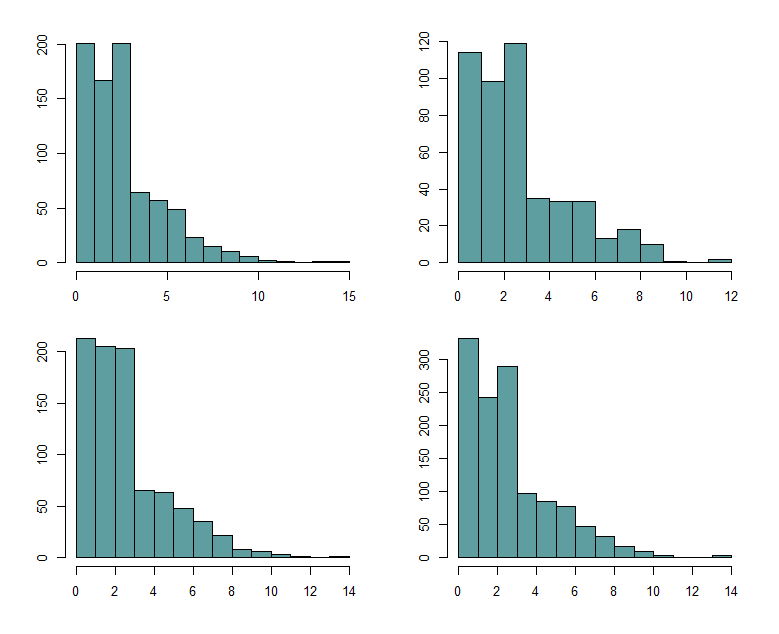
\includegraphics[scale=0.7]{../Slike za rad/Skupine.png}
\end{center}
\caption{Хистограми одабраних скупина}
\label{skupp}
\end{figure}

Кластер узорак заснован на извлачењу скупина са понављањем формиран је у скрипту \ref{sscswr}. За разлику од верзије без понављања, где су групе узорковане простим случајним узорковањем, овде је то учињено узорковањем са неједнаким вероватноћама, сразмерним величини скупине. Прецизност класификације је 89,68 \%, практично најбоља досад, док су дисперзије оцена упоредиве са ранијим покушајима, уз напомену да се Хансен-Хурвицова оцена показала као врло прецизна, што не иде у прилог претпоставци, али би се могло објаснити тиме да су групе одлично одабране, што и приказују приложени хистограми.

\lstinputlisting[caption={sscswr.r -- модел над групним узорком са пон.},label=sscswr]{../R skriptovi/sscswr.r}

По обичају, на крају је изложено шта се дешава када је лоше примењен текући план узорковања. Тако је кластер узорак -- прост случајан без понављања и са неједнаким вероватноћама и понављањем -- такав да групе не испуњавају претпоставке метода, формиран у скрипту \ref{sscslos}.

\lstinputlisting[caption={sscslos.r -- модел над лошим групним узорком},label=sscslos]{../R skriptovi/sscslos.r}

Кластеровање је извршено према типу слова, као да је у питању стратификација. То је резултовало групама које, за разлику од претходног приступа, нису довољно сличне, а међусобно су различите, о чему сведоче хистограми на слици \ref{skupl}. Отуда су и процењене дисперзије свих предложених оцена вишеструко веће. Како је критеријум груписања био тип слова, класификациони модел није могао да научи особине више од четири обухваћене групе, тако да је удео погодатака свега 15-16 \%, што управо и јесте блиско очекивању $\frac{4}{26} \approx 0,1538$.

\begin{figure}[h!]
\begin{center}
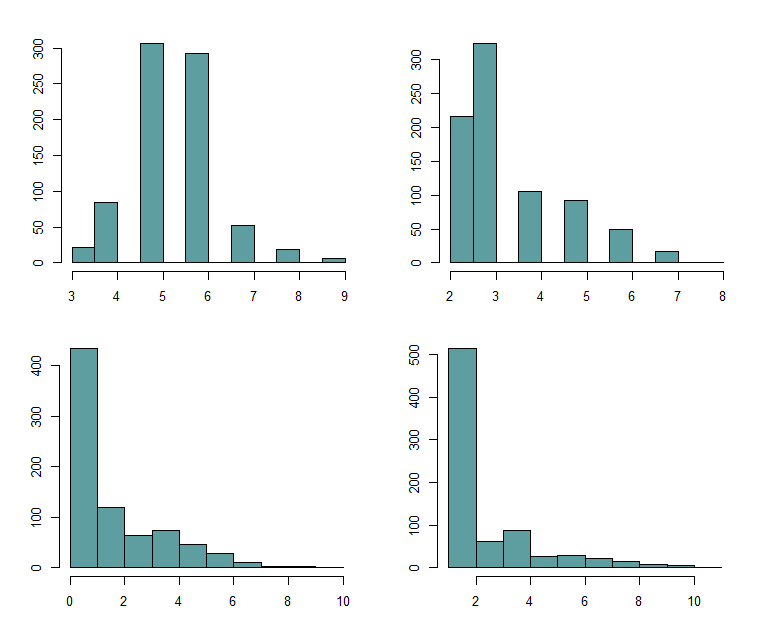
\includegraphics[scale=0.57]{../Slike za rad/Skupinel.png}
\end{center}
\caption{Хистограми одабраних скупина}
\label{skupl}
\end{figure}

Сумарно, закључак је да је први део хипотезе тачан -- стварно нема негативног утицаја јефтинијег групног узорковања на прецизност класификационог модела. С друге стране, други део претпоставке зависи од квалитета кластеровања. Уколико су скупине довољно репрезентативне, као популације у малом, прецизност оцена је слична или боља него код простог случајног узорка. Постојаност је слабија тек када важи супротно. Ово је у складу са уводним теоријским разматрањем.

\subsection{Систематски узорак}

Систематски узорак је изразито једноставан план узорковања, једноставнији чак и од простог случајног узорка, који у основи има исту структуру као једноетапни групни узорак.\cite{prez9} Свака примарна јединица састоји се од секундарних јединица које су на известан систематски начин распоређене широм популације. Најједноставнији случај представља прост систематски узорак, такође назван периодични или механички узорак, код кога је свака скупина фактички низ индекса са кораком. Под претпоставком да важи $N = nK$, величина $K$ назива се корак, односно период(а) узорка. Према систематском плану узорковања, бира се тачно једна примарна јединица, па тако он одговара групном узорку обима један, и то на следећи начин -- од првих $K$ секундарних јединица одабере се једна као почетна, а затим свака $K$-та, чиме се добија жељени узорак величине $n$ или евентуално са неким ентитетом мање, уколико није у питању целобројни умножак.

Највећа предност оваквог плана узорковања јесте његова донекле банална једноставност, као и ниска цена и економичност. Добра особина је и што постоји мањи укупан број узорака него код простог случајног узорка (тачно $K$), при чему не постоје преклапања секундарних јединица у узорцима, па је тако лако израчунати нпр. вероватноће укључења сваке инстанце. Генерисање (псеудо)случајних бројева неопходно је само једанпут, за одабир почетне инстанце. Потпуна енумерација ентитета у популацији није потребна ни у једном тренутку. Још неке интуитивне предности систематског узорка јесу равномерна расподела на популацији, као и чињеница да не допушта случајна груписања или пропуштање заступљености неких делова популације.

Као тачкаста оцена популацијске средње вредности може се користити узорачка средња вредност. Њена дисперзија, међутим, одређена са $\frac{1}{n^2K} \sum_{l=1}^K (\tau_l - \frac{\tau_y}{K})^2$, није једноставна за процену на основу узорка, што је главно ограничење у примени систематског узорка. Коришћењем класичне формуле за оцену дисперзије код групног узорка обима један добила би се бескорисна процена нула. Срећом, проблем је могуће превазићи добрим познавањем проучаване популације. Под претпоставком да су ентитети случајно распоређени по популацији, односно да не постоји веза између индекса јединке и вредности обележја од значаја на њој, могуће је применити оцену која важи код простог случајног узорка без понављања. Овако је са проучаваним скупом слова, па се могу очекивати исти резултати као на почетку. С друге стране, када подаци показују монотону или периодичну везу са индексима, онда се систематски узорак може показати као знатно бољи или гори.

\begin{hipoteza}
Класификациони модел направљен над систематским узорком скупа слова једнаког је успеха као онај направљен над простим случајним узорком, а исто важи и за прецизност оцена.
\end{hipoteza}

Периодични систематски план узорковања примењен је у скрипту \ref{sys}. Како је и претпостављено, за исти обим узорка, сви резултати су скоро идентични оним код простог случајног узорка -- прецизност класификационог модела, вредност и прецизност оцена. Ово је у складу са запажањем из теоријског увода да је систематски узорак над добро промешаној популацији (у смислу расподеле обележја од интереса) заправо јефтинија верзија простог случајног узорка без понављања.

\lstinputlisting[caption={sys.r -- модел над систематским узорком},label=sys]{../R skriptovi/sys.r}

\subsection{Вишеетапни узорак}

Поред једноетапног групног узорка, постоји и вишеетапна варијанта истог плана узорковања.\cite{prez10} Наиме, једноетапна верзија, иако веома једноставна, може бити непрактична у случају великих група. Ентитети који сачињавају скупине могу бити толико слични да испитивање свих представља разбацивање ресурса. Кластери су као мале популације, па испитивање сваког члана не повећава значајно репрезентативност узорка, а прави додатан трошак који са собом носи регистровање вредности обележја на секундарним јединицама.

Најпростија верзија овог плана јесте двоетапни узорак, код кога се у првој етапи одабере одређени број примарних јединица, а затим се из сваке одабере подузорак секундарних јединица. У обе етапе је произвољан метод одабира, с тим што је у другој то најчешће прост случајан узорак без понављања. Ознаке и оцене остају исте као код једноетапног кластеровања, с тим што се додатно уводи $n_l$ као обим подузорка $l$-тог кластера, који сада није једнак величини целе скупине. Код оцена је још неопходно проценити тотал за сваки извучени кластер, за шта се користе непристрасне оцене метода примењеног у другој фази. Дисперзије су нешто веће него код једноетапне верзије, с тим што се додатни други сабирак често може одбацити као занемарљиво мали у односу на први, који постоји код обе варијанте.

\begin{hipoteza}
Класификациони модел направљен над двоетапним групним узорком једнако је прецизан као онај направљен над једноетапним, када су групе изабране на исти начин. Резултујуће оцене популацијске средње вредности сличне су постојаности.
\end{hipoteza}

Двоетапни узорак заснован на извлачењу скупина без понављања формиран је у скрипту \ref{mscswor}. Групе су у првој етапи формиране на исти начин као код једноетапне верзије, док је у другој примењен прост случајан узорак без понављања. Запажања су једнака као код верзије са само једном етапом, што иде у прилог изложеној претпоставци.

\lstinputlisting[caption={mscswor.r -- модел над двоетапним узорком без пон.},label=mscswor]{../R skriptovi/mscswor.r}

Двоетапни узорак заснован на извлачењу скупина са понављањем формиран је у скрипту \ref{mscswr}. Као код једноетапне варијанте, за разлику од верзије без понављања, где су групе узорковане простим случајним узорковањем, овде је то у првој етапи учињено узорковањем са неједнаким вероватноћама, сразмерним величини скупине, док је у другој такође примењен прост случајан узорак без понављања. И овде су запажања као код верзије са једном етапом, макар по питању класификације, пошто дисперзије због комплексности нису процењиване.

\lstinputlisting[caption={mscswr.r -- модел над двоетапним узорком са пон.},label=mscswr]{../R skriptovi/mscswr.r}

И сада је крају изложено шта се дешава када је лоше примењен текући план узорковања. Тако је двоетапни узорак -- прост случајан без понављања и са неједнаким вероватноћама и понављањем у првој, а прост случајан без понављања у другој етапи -- такав да групе не испуњавају претпоставке метода, формиран у скрипту \ref{mscslos}. Кластери су формирани на исти начин као раније -- према типу слова. Још једном, утисци су непромењени у односу на варијанту са једном етапом.

\lstinputlisting[caption={mscslos.r -- модел над лошим двоетапним узорком},label=mscslos]{../R skriptovi/mscslos.r}

\section{Закључак}

Узорковање је важан поступак у раду са подацима, поготову оним великог обима. Над скупом ентитета који представљају велика слова енглеске абецеде примењено је неколико планова узорковања, са посебном пажњом усмереном на познати проблем класификације.

Након детаљног описа података, прво су примењене методе простог случајног узорка и узорка са неједнаким вероватноћама извлачења. Том приликом је потврђена претпоставка да су бољи модели направљени над подацима код којих је очувана расподела обележја високе погађачке моћи. Ово је послужило за формулацију новог статистички заснованог начина одређивања важности предиктора.

Затим је испитана и потврђена претпоставка да модели направљени над скупом података из кога су искључена висококорелисана обележја (вертикални узорак) постижу сличан успех као они направљени над целим скупом, док искључивање некорелисаних обележја смањује прецизност, уз напомену да то важи уз одређени степен грешке.

Показана је важност раслојавања тј. обраћања пажње на добар удео категорија у подацима на основу којих се прави класификациони модел, као и чињеница да је стратификовани узорак углавном бољи за процену популацијских вредности од простог случајног узорка.

Испитано је и да ли јефтинији план узорковања нужно даје лошије резултате и потврђено је да није тако -- једноетапни групни узорак код кога су групе добро одабране (унутар себе различите, као популација у малом, а међусобно сличне) дао је не само добре резултате класификације, већ и најразличитије оцене високе прецизности. Подједнако добро понашање показао је и двоетапни узорак са истим скупинама и дупло мањим обимом, као и периодични систематски узорак.

Када је у питању оцењивање средње вредности обележја од значаја (четрнаестог атрибута), уз закључивање засновано на методу одабира узорка, најбољу оцену у смислу прецизности/постојаности дало је количничко оцењивање код једноетапног групног узорка -- процењена варијанса 0,0003. Иако прецизна, ова оцена је пристрасна. Код истог плана узорковања, дисперзија је процењена на високих 0,2419 када се користи непристрасна оцена. Сви прости случајни узорци (без понављања, са понављањем, редуковани са понављањем) дали су оцену чија је дисперзија процењена као 0,0014. Неједнаке вероватноће са понављањем условиле су Хансен-Хурвицову оцену дисперзије 0,0033 и Хорвиц-Томпсонову 0,0058 за редуковани узорак. Раслојено узорковање по типу слова са Нејмановим оптималним распоредом и простим случајним узорком без понављања као позадинским приступом резултовало је дисперзијом оцене од нешто испод 0,0005. Како је ово најмања варијанса код једне тачне (непристрасне и постојане) оцене, она је најбоља у средњеквадратном смислу. Постстратификација простог случајног узорка није донела побољшања због релативно униформне расподеле типа слова. Код једноетапног групног узорка са понављањем и неједнаким вероватноћама избора сразмерним величини кластера дисперзија Хансен-Хурвицове оцене процењена је као добрих 0,0008, а Хорвиц-Томпсонове као нешто лошијих 0,0113. Варијансе код двоетапног кластер узорка са истим скупинама биле су врло сличне. Систематски узорак био је еквивалентан простом случајном узорку без понављања, са процењеном дисперзијом оцене око 0,0015.

Даље истраживање могло би да се фокусира на додатну и ригорознију проверу хипотеза изнесених у раду, нпр. на већем броју различитих база података или пак другим обележјима скупа слова. Осим тога, не би било лоше испитати успешност нешто сложенијих планова узорковања, као што је двофазни план. У том случају би у првој фази било могуће сакупити додатне значајне информације о популацији, које би олакшале другу, главну фазу, слично пилот истраживању које је спроведено за одређивање обима простог случајног узорка.

\newpage
\addcontentsline{toc}{section}{Литература}
\appendix
\bibliography{Uzorko\string~1}
\bibliographystyle{unsrt}

\end{document}
